
\chapter{Equivalent Circuits}

\section{Intro}
Intro stuff goes here.

\section{The Electric Field}

Suppose there are two particles of charge $q_1$ and $q_2$ located a distance $r_{12}$ apart.
The force on particle 2 is given by:
\begin{displaymath}
\vec{F}_{12} = k_e \frac{q_1 q_2}{r_{12}^2} \cdot \hat{r}_{12}
\end{displaymath}
where $k_e$ is Coulomb's constant and $\hat{r}_{12}$ is a unit vector pointing from particle 1 to particle 2.

Now consider the force $\vec{F}$ on a particle of charge $Q$ due to $N$ particles, which will be the sum:
\begin{displaymath}
\vec{F} = Q \, k_e \, \sum_{i=1}^N \frac{q_i}{r_{i}^2} \hat{r}_{i}
\end{displaymath}
where $r_i$ is the distance between the particle of charge $Q$ and the $i$th particle, and $\hat{r}_i$ is the unit vector pointing from the $i$th particle toward the charge $Q$.  The ratio of the force $F$ to the charge $Q$ is independent of the charge $Q$, and we call this quantity the electric field:
\begin{displaymath}
\vec{E} \equiv \frac{\vec{F}}{Q}
\end{displaymath}
The importance of this distinction is that the electric field is due solely due to the source charges, independent of the particle of charge $Q$ experiencing the force.  The electric field exists whether or not anything is there to experience a force!  The force experienced by a particle of charge $Q$ in an electric field $\vec{E}$ is given by:
\begin{displaymath}
\vec{F} = Q \vec{E}.
\end{displaymath}

\section{The Electric Potential}

For a conservative force the change in potential energy that results from moving a particle from $x=a$ to $x=b$ is defined as the negative of the work done by the conservative force:
\begin{displaymath}
U_{ab} \equiv -W_{\rm CSV} = - \int_a^b F_x \cdot dx
\end{displaymath}
As discussed above, the Coulomb force $\vec{F}$ experienced by a 
particle of charge $Q$ in an electric field $\vec{E}$ is given by:
\begin{displaymath}
\vec{F} = Q \vec{E} 
\end{displaymath}
which is a conservative force proportional to the charge $Q$.   If we consider moving a particle of charge $Q$ moving along the $x$-axis from $x=a$ to $x=b$, we can define a quantity $V_{ab}$ called the electric potential difference which is simply the change in potential energy divided by the charge of the particle:
\begin{displaymath}
V_{ab} \equiv \frac{U_{ab}}{Q}  = - \int_a^b E_x \cdot dx
\end{displaymath}
The unit of electrical potential difference is the Volt (V), where $1~\rm{V} = 1~\rm{J / C}$, and a difference in electrical potential is often informally referred to as simply the voltage.  This definition generalizes to three dimensions, but is tedious (you simply add additional identical integrals for $y$ and $z$) without vector calculus, which we won't use in this  course.   In this case the points $b$ and $a$ are simply any two points in space.

\begin{figure}[htbp]
\begin{center}
\begin{tabular}{ccc}
\begin{circuitikz}[line width=1pt]
\draw (0,2) to[battery1] ++(0,-2.0);
\draw (0,0.7) node[left]{$-$};
\draw (0,1.4) node[left]{$+$};
\end{circuitikz} &  
\begin{circuitikz}[line width=1pt]
\draw (0,2) to[battery] ++(0,-2.0);
\draw (0,0.5) node[left]{$-$};
\draw (0,1.6) node[left]{$+$};
\end{circuitikz} & 
\begin{circuitikz}[line width=1pt]
\draw (0,0) to[voltage source, bipoles/length=1.5cm] ++(0,+2.0);
\end{circuitikz} \\
(a) & (b) & (c) \\
\end{tabular}
\end{center}
\caption{The circuit diagram for (a) voltage cell, (b) battery, (c) voltage source.  The $+$ and $-$ symbols are usually omitted from (a) and (b).  Often, symbol (a) is used to indicate a generic voltage source, even when (c) would be more appropriate.}
\label{fig:dcsymbols}
\end{figure}


\begin{figure}[htbp]
\begin{center}
\begin{tabular}{cc}
\begin{circuitikz}[line width=1pt]
\draw (0,0) node[ground, yscale=2.0]{};
\end{circuitikz}  & 
\begin{circuitikz}[line width=1pt]
\draw (0,0) coordinate(A) to[voltage source,bipoles/length=1.5cm,l_=3~\rm V] ++(0,+2.0)
coordinate(B) to[voltage source,bipoles/length=1.5cm,l_=2~\rm V] ++(0,+2.0) coordinate(C);
\draw (A) to[short,-o] ++(1.0,0) node[right]{A};
\draw (B) to[short,-o] ++(1.0,0) node[right]{B};
\draw (C) to[short,-o] ++(1.0,0) node[right]{C};
\draw (A) node[ground, yscale=2.0]{};
\end{circuitikz} \\
(a) & (b) \\
\end{tabular}
\end{center}
\caption{The (a) ground symbol, and (b) circuit diagram for two voltage sources connected in series and referenced to ground.}
\label{fig:poteg}
\end{figure}

The battery is a frequently encountered electrical component that imposes a constant electrical potential difference between two points (the two terminals of the battery).  Batteries are devices that exploit different chemical potentials of two metals.  A cell consisting of zinc and copper will have a characteristic voltage of $1.1~\rm V$.  To build batteries of different voltages, multiple cells can be combined.  In lab, you will use a bench-top DC voltage supply, a more complicated piece of equipment that uses electrical power provided by the wall outlets to maintain a fixed voltage between its terminals.  All real devices have limitations.  For instance, batteries drop in voltage as they become discharged.  

Because these devices supply a fixed voltage which is approximately constant with time, they produce circuits with currents in one direction only.   As a result, these are called direct current (DC) sources.
The electrical symbols for various DC voltage sources are shown in Fig.~\ref{fig:dcsymbols}

By definition, a conservative force has a single value for the relative potential $U_{ab}$ which is independent of the path taken from point $a$ to point $b$.   The same holds for $V_{ab}$.
This implies that $V_{ab} = -V_{ba}$ which is why terminals of any voltage source have a polarity.  If we specify a reference point, we can define the electrical potential as the electrical potential difference of the point of interest and the reference point.   Most often, the reference point chosen is the earth ground, which has it's own symbol, shown in Fig.~\ref{fig:poteg}a.  In the circuit diagram of Fig.~\ref{fig:poteg}b, examples of electrical potential differences are $V_{\rm AB} = 3~{\rm V}$, $V_{\rm BC} = 2~{\rm V}$,  and $V_{\rm BA}= -3~{\rm V}$, while examples of electrical potentials are $V_A = 0$, $V_B = 3~\rm V$ $V_C = 5~\rm V$.

\section{Conductors and Resistors}

The electric field in a perfect conductor is zero.  This implies that any two points connected by a perfect conductor are at the same electric potential, which we refer to as a short circuit.  As a practical matter, we treat very good conductors, such as copper, as if they were ideal conductors.  We create a short circuit by connecting any two points with a segment of copper wire.   Conductors allow charge to flow through them readily.   The amount of charge that passes through any electrical component per unit time is called the current $I$:
\begin{displaymath}
I = \frac{dQ}{dt}
\end{displaymath}
And is measured in Amperes (A) where $1~{\rm A} = 1 {\rm C / s}$.

Materials which do not readily conduct charge are called electrical insulators, and are used to protect components, such as wires, from accidental contact causing unintentional short circuits.  All materials eventually conduct electricity when the voltage is high-enough, and this imposes limits on the voltage that can be reached in practical circuits.

\begin{figure}[htbp]
\begin{center}
\begin{circuitikz}[line width=1pt]
\draw (0,0) to[voltage source,bipoles/length=1.5cm,l=$V$] ++(0,+3.0) to[short,i>=$I$] ++(3.0,0) coordinate(A)
to[resistor,l_=$R$] ++(0,-3.0) coordinate(B) to[short] ++(-3.0,0);
\draw (A) to[short,*-o] ++(1.0,0) node[right]{A};
\draw (B) to[short,*-o] ++(1.0,0) node[right]{B};
\end{circuitikz} 
\end{center}
\caption{A resistor connected to a voltage source.}
\label{fig:ohms}
\end{figure}

If we construct a composite material from a mixture of graphite (a conductor) and ceramic dust (an insulator) held together by a resin, we obtain a resistor: a device which has mobile charges that do not flow as readily as in a conductor.  When we connect a resistor to a voltage source,  as shown in Fig.~\ref{fig:ohms}, 
the voltage source imposes a non-zero electric potential across the resistor.  This implies that a non-zero electric field is present in the resistor.  This electric field exerts a force on the mobile electrons in the resistor, resulting in a net flow of electrons through the resistor.  Resistors have a characteristic resistance $R$ which relates the current $I$ that flows through the resistor to the voltage $V$ across it: 
\begin{displaymath}
V = I R
\end{displaymath}
This relationship is referred to as Ohm's Law, and the unit of resistance is the Ohm ($\rm \Omega$) where $1~{\rm \Omega} = 1~{\rm V / A}$.

\section{Kirchhoff's Laws}

The circuits we have encountered so far are quite simple, containing at most a single closed loop with only one current to consider.  More complicated circuits can include multiple circuits.
Ultimately the behavior of the circuit is governed by the laws of electrostatics, but Kirchhoff's Laws conveniently cast the important results from electrostatics into a form that can be applied to any circuit.

\begin{figure}[htbp]
\begin{center}
\begin{circuitikz}[line width=1pt]
\draw (0,0) to[short,i>=$I_1$,-*] ++(1.4,1.4) coordinate(C);
\draw (C) to[short,i>=$I_3$] ++(1.4,-1.4);
\draw (C) to[short,i<=$I_2$] ++(0,2);
\end{circuitikz} 
\end{center}
\caption{An example of Kirchoff's Current Law:  $I_1 + I_2 = I_3$}.
\label{fig:kcleg}
\end{figure}


The conservation of charge implies that the total current into a node must equal the total current out of a node.  If currents are all defined such that positive current is into the node, this law can be written simply as:
\begin{displaymath}
\sum_k I_k = 0.
\end{displaymath}
This is referred to as Kirchhoff's Current Law (KCL).

The electric field is conservative which implies that the net electric potential when traversing any closed loop is zero.  If the voltage drop across each electric component is defined in the direction of the closed loop, this law can be written simply as:
\begin{displaymath}
\sum_k V_k = 0.
\end{displaymath}
This is referred to as Kirchhoff's Voltage Law (KVL).  When determining the drop across a resistor from Ohm's law, one must remember the orientation of current and voltage (as in Fig.~\ref{fig:ohms}) when determining the sign.  You should be able to reason that when traversing a resistor in the same direction as the current, you drop in voltage (so add a term $-IR$ when using KVL).  When traversing a resistor in the opposite direction as the current, you rise in voltage (so add a term $IR$ when using KVL.) 

\begin{figure}[htbp]
\begin{center}
\begin{circuitikz}[line width=1pt]
\draw (0,0) to[voltage source,bipoles/length=1.5cm,l=$V$] ++(0,+3.0) to[resistor,l=$R_1$,i>=$I_1$] ++(3.0,0) coordinate(A) to[resistor,l=$R_2$,i>=$I_2$] ++(0,-3.0) coordinate(B) to[short] ++(-3.0,0);
\draw (A) to[R,*-,l=$R_3$,i>=$I_3$] ++(3.0,0) |- (B);
\draw (1.5,1.5) coordinate(L) node[scale=4]{$\circlearrowright$};
\draw (L) node[]{$1$};
\draw (4.5,1.5) coordinate(L) node[scale=4]{$\circlearrowright$};
\draw (L) node[]{$2$};
\end{circuitikz} 
\end{center}
\caption{An example of Kirchoff's Voltage Law.}
\label{fig:kvleg}
\end{figure}

For example, consider the circuit in Fig.~\ref{fig:kvleg}.  From KCL we obtain:
\begin{displaymath}
I_1 = I_2 + I_3
\end{displaymath}
while from KVL we traverse the loop labeled "1" to obtain:
\begin{displaymath}
0 = V  - I_1 R_1 - I_2 R_2
\end{displaymath}
and we traverse the loop labeled "2" to obtain
\begin{displaymath}
0 = I_2 R_2 - I_3 R_3
\end{displaymath}
Pay close attention to the signs of the voltage drops across the resistors and make sure you can reproduce them!



\section{Resistors in Series And Parallel}

\begin{figure}[htbp]
\begin{center}
\begin{tabular}{c@{\hskip 2cm}c}
\begin{circuitikz}[line width=1pt]
\draw (0,0) to[voltage source,bipoles/length=1.5cm,l=$V$] ++(0,+4.0) to[short, i>=$I$] ++(2.0,0) coordinate(A);
\draw (A) to[resistor,l_=$R_1$] ++(0,-2.0) to[resistor,l_=$R_2$] ++(0,-2.0) to[short] ++(-2.0,0);
\end{circuitikz} &
\begin{circuitikz}[line width=1pt]
\draw (0,0) to[voltage source,bipoles/length=1.5cm,l=$V$] ++(0,+4.0) to[short, i>=$I$] ++(2.0,0) coordinate(A);
\draw (A) to[resistor,l=$R_{\rm eq}$] ++(0,-4.0) to[short] ++(-2,0);
\end{circuitikz} \\
(a) & (b) \\
\end{tabular}
\caption{Resistor circuits showing (a) two resistors in series and (b) a single equivalent resistance $R_{\rm eq} = R_1 + R_2$ which produces the same current $I$.}
\label{fig:series}
\end{center}
\end{figure}

Consider the circuit in Fig.~\ref{fig:series} in which a current $I$ flows through to resistors $R_1$ and $R_2$ in series.  We can simplify this circuit by determining a single equivalent resistance $R_{\rm eq}$ which when installed in the circuit in place of $R_1$ and $R_2$ will result in the same current $I$.
Applying KVL to both circuits results in:
\begin{eqnarray*}
0 &=& V - I R_1 - I R_2 \\
0 &=& V - I R_{\rm eq} \\
\end{eqnarray*}
which can be solved to obtain:
\begin{displaymath}
R_{\rm eq} = R_1 + R_2.
\end{displaymath}
It is left as an exercise to show that for any number of resistors wired in series, the equivalent resistance
is given by:
\begin{equation} \label{eqn:rseries}
R_{\rm eq} = \sum_i R_i. 
\end{equation}

\begin{figure}[htbp]
\begin{center}
\begin{tabular}{c@{\hskip 2cm}c}
\begin{circuitikz}[line width=1pt]
\draw (0,0) to[voltage source,bipoles/length=1.5cm,l=$V$] ++(0,+4.0) to[short,i>=$I$] ++(2.0,0) coordinate(A);
\draw (A) to[resistor,l_=$R_1$,i>=$I_1$] ++(0,-4.0) to[short] ++(-2,0);
\draw (A) to[short,*-] ++(2.0,0.0) to[resistor,l_=$R_2$,i>=$I_2$] ++(0.0,-4.0) to[short,-*] ++(-2.0,0);
\end{circuitikz} &
\begin{circuitikz}[line width=1pt]
\draw (0,0) to[voltage source,bipoles/length=1.5cm,l=$V$] ++(0,+4.0) to[short,i>=$I$] ++(2.0,0) coordinate(A);
\draw (A) to[resistor,l=$R_{\rm eq}$] ++(0,-4.0) to[short] ++(-2,0);
\end{circuitikz} \\
(a) & (b) \\
\end{tabular}
\caption{Resistor circuits showing (a) two resistors in parallel and (b) a single equivalent resistance $R_{\rm eq}$ which produces the same total current $I$.}
\label{fig:parallel}
\end{center}
\end{figure}

Next consider the circuit in Fig.~\ref{fig:series} in which a total current $I$ is shared between two resistors $R_1$ and $R_2$.  Once again, we can simplify this circuit by determining a single equivalent resistance $R_{\rm eq}$ which when installed in the circuit in place of $R_1$ and $R_2$ will result in the same current $I$.  Applying KCL and KVL we determine:
\begin{eqnarray*}
I &=& I_1 + I_2 \\
0 &=& V - I_1 R_1 \\
0 &=& V - I_2 R_2 \\
0 &=& V - I R_{\rm eq} \\
\end{eqnarray*}
which can be solved to determine:
\begin{displaymath}
R_{\rm eq} = \frac{R_1 R_2}{R_1 + R_2}
\end{displaymath}
It is left as an exercise to show that for any number of resistors wired in parallel, the equivalent resistance
is given by:
\begin{equation} \label{eqn:rparallel}
\frac{1}{R_{\rm eq} }= \sum_i \frac{1}{R_i}. 
\end{equation}

\begin{figure}[htbp]
\begin{center}
\begin{tabular}{c@{\hskip 2cm}c}
\begin{circuitikz}[line width=1pt]
\draw (0,0) node[ground,yscale=2.0]{} to[voltage source,bipoles/length=1.5cm,l=$V$] ++(0,+4.0) to[short,i>=$I$] ++(2.0,0) coordinate(A);
\draw (A) to[resistor,l_=$R_1$] ++(0,-2.0) coordinate(B) to[resistor,l_=$R_2$] ++(0,-2.0) to[short] ++(-2.0,0);
\draw (B) to[short,*-o] ++(1.0,0) node[right]{$V_{\rm out}$};
\end{circuitikz} &
\begin{circuitikz}[line width=1pt]
\draw (0,0) node[ground,yscale=2.0]{} to[voltage source,bipoles/length=1.5cm,l=$V$] ++(0,+4.0) to[short,i=$I$] ++(2.0,0) coordinate(A);
\draw (A) to[resistor,l_=$R_1$,i>=$I_1$] ++(0,-4.0) to[short] ++(-2,0);
\draw (A) to[short,*-] ++(2.0,0.0) to[resistor,l_=$R_2$, i>=$I_2$] ++(0.0,-4.0) to[short,-*] ++(-2.0,0);
\end{circuitikz} \\
(a) & (b) \\
\end{tabular}
\caption{Resistors in series and in parallel used to implement a (a) voltage divider and a (b) current divider.}
\label{fig:dividers}
\end{center}
\end{figure}

The voltage divider circuit of Fig.~\ref{fig:dividers}a is a frequently encountered circuit.  The two resistors have an equivalent resistance $R_1 + R_2$ and so the current is:
\begin{displaymath}
I = \frac{V}{R_1 + R_2} 
\end{displaymath}
and the output voltage is the voltage drop across one resistor $R_2$, 
\begin{displaymath}
V_{\rm out} = I R_2 = \frac{R_2}{R_1 + R_2} V
\end{displaymath}
It is left as an exercise to show that the current divider circuit in Fig.~\ref{fig:dividers}b 
\begin{equation} \label{eqn:idivider}
\frac{I_1}{I_2} = \frac{R_2}{R_1}
\end{equation}

\section{The Superposition Principle}

In electrostatics, the superposition principle states that the electric field created at a point in space by a particular charge is independent of any other charges.  This principle allows us to simplify problems in electrostatics by considering the contribution from each charge in turn, constructing a partial solution for each charge while neglecting other charges, and constructing a solution from the sum of each partial solution.

In circuit analysis, the laws of electrostatics govern our circuits as well.  When considering a circuit with multiple voltage sources, we can consider one voltage source at a time, short circuiting other voltage sources.  The complete solution is simply the sum of each partial solution.

\section{Sources, Loads, $I$-$V$ Curves, and Power}

Analyzing complicated circuits inevitably involves breaking them down into smaller parts that are more easily understood.   A particularly useful way to divide circuits is in terms of sources and loads.  Consider first the simple circuit consisting of a voltage source connected to a resistor.  As illustrated in Fig.~\ref{fig:source_load}, both the voltage source and the resistor can be considered as two separate two terminal networks.  If we wish to connect these two networks together, we must agree on a definition for the direction of the current $I$.  One of the networks will have positive current $I$ leaving the positive terminal (A), and we call this network the ``source".  The other network will have positive current entering the positive terminal, and we call this network the ``load".  

\begin{figure}[htbp]
\begin{center}
\begin{tabular}{cc}
\begin{circuitikz}[line width=1pt]
\draw (0,0) node[right]{A} to[short,o-] ++(-1.0,0) to[voltage source,bipoles/length=1.5cm,l=$V_1$] ++(0,+4.0) to[short, i>=$I$,-o] ++(1.0,0) node[right]{B};
\draw (1, 0.0) to [open,v_>=$V$] (1,4.0);
\end{circuitikz} &
\begin{circuitikz}[line width=1pt]
\draw (0,0) node[left]{A} to[short,o-] ++(1.0,0) to[R,l=$R_1$] ++(0,+4.0) to[short, i<=$I$,-o] ++(-1.0,0) node[left]{B};
\end{circuitikz} \\
(a) & (b) \\
\end{tabular}
\caption{ Two terminal network diagrams for (a) an ideal voltage as a source, and (b) as a resistor as load.}
\label{fig:source_load}
\end{center}
\end{figure}

When considered separately, we can imagine connecting various resistors or even additional batteries to the two terminal voltage source.  However, as long as we don't do anything that breaks the voltage source, it will keep the voltage between A and B at the fixed value $V_1$ no matter what we do, providing any amount of current needed.  We can also consider connecting batteries of different sizes to the two-terminal load network.  In this case, the resistor will allow a current to flow consistent with Ohm's law, in this case:  $V = I R_1$.  We can consider both the source network and load network as having separate curves in the 
$I$-$V$ plane, as shown in Fig.~\ref{fig:vr_iv} .  The source curve is the vertical line $V=V_1$ while the load curve is a line of slope $1/R_1$ with zero intercept.

The intersection of the source $I$-$V$ curve with the load $I$-$V$ curve is the operating point for the circuit that results form connecting the load to the source.  A source providing a current $I$ while maintaining  a potential difference $V$ across it's two terminals is powering the circuit with power:
\begin{displaymath}
P \equiv \frac{dU}{dt} = \frac{VdQ}{dt} = V \frac{dQ}{dT} = V I
\end{displaymath}
Meanwhile, the load is consuming power $P = VI$.  It is instructive to consider what would happen if you called the voltage source the load and the resistor the source.  In this case, the current simply changes sign, and you would find that at the operating point the so-called supply is providing negative power.  In other contexts you might find that both the current $I$ and the voltage $V$ are negative, so that the power provided by the source is positive.  In this case, you have likely correctly identified the roles of source and load while making a poor choice for the polarity.

\begin{figure}[htbp]
\begin{center}
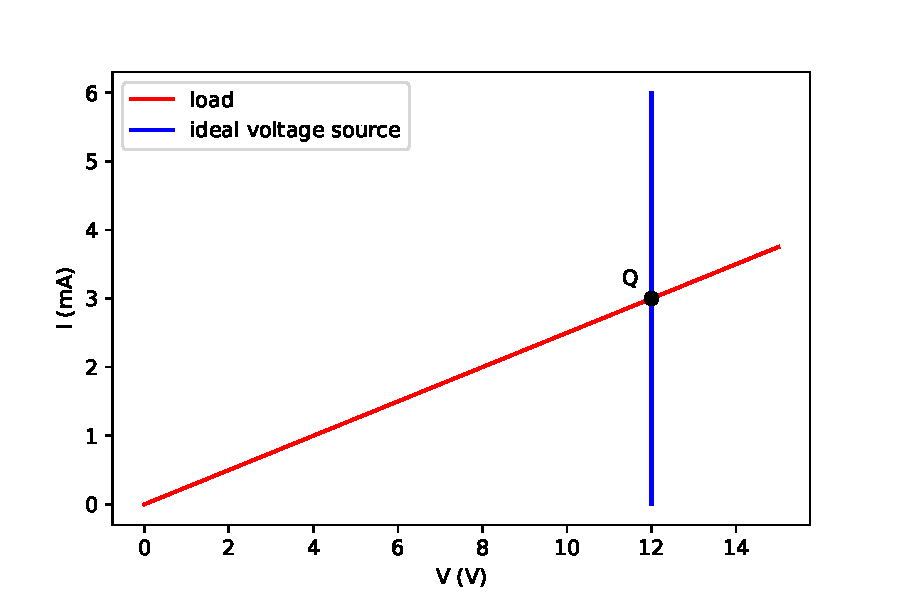
\includegraphics[height=0.3\textheight]{figs/thev_ideal.pdf} \\
\caption{ The source $I-V$ curve for an ideal $12~\rm V$ voltage source, and the load $I-V$ curve for a $4~\rm k\Omega$ resistor.   The operating point for the circuit when the load is connected to the source is the intersection of these two curves at point $Q$.  The power provided by the source and consumed by the load is the product $IV$ at the operating point.}
\label{fig:vr_iv}
\end{center}
\end{figure}

\begin{figure}[htbp]
\begin{center}
\begin{tabular}{cc}
\begin{circuitikz}[line width=1pt]
\draw (0,0) node[right]{A} to[short,o-] ++(-1.0,0) to[voltage source,bipoles/length=1.5cm,l=$V_1$] ++(0,+2.0) 
to[R, l=$R_{\rm src}$] ++(0,+2.0) to[short, i>=$I$,-o] ++(1.0,0) node[right]{B};
\draw (1, 0.0) to [open,v_>=$V$] (1,4.0);
\end{circuitikz} &
\begin{circuitikz}[line width=1pt]
\draw (0,0) node[left]{A} to[short,o-] ++(1.0,0) to[R,l=$R_1$] ++(0,+4.0) to[short, i<=$I$,-o] ++(-1.0,0) node[left]{B};
\end{circuitikz} \\
(a) & (b) \\
\end{tabular}
\caption{ Two terminal network diagrams (a) for a voltage source include source resistance $R_{src}$ as the source, and (b) a load resistor.}
\label{fig:vrr}
\end{center}
\end{figure}

\begin{figure}[htbp]
\begin{center}
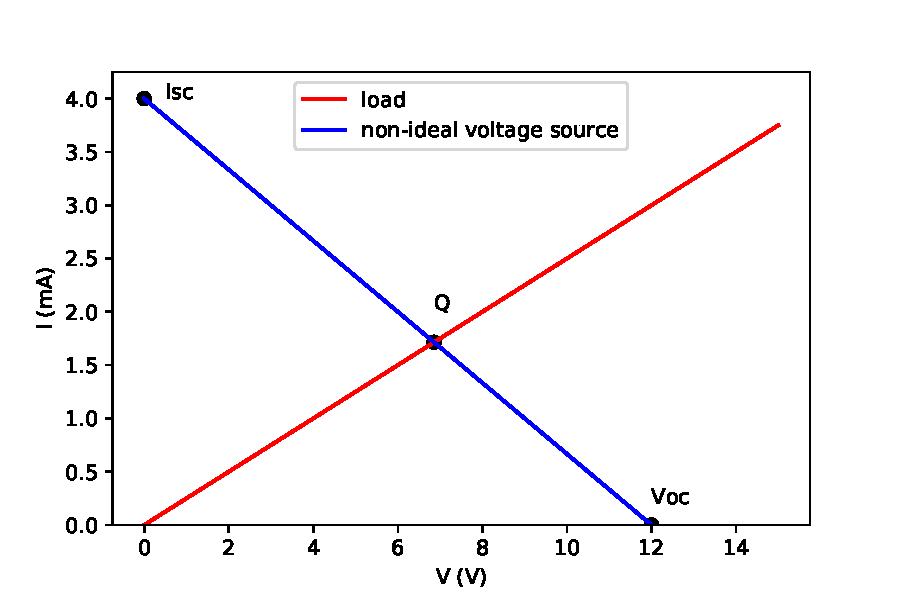
\includegraphics[height=0.3\textheight]{figs/thev_nonideal.pdf} \\
\caption{ $I-V$ curves for a non-ideal $12~\rm V$ source which includes a source resistance of $R_{\rm src} = 3~\rm k\Omega$ and a load resistance of $4~\rm k\Omega$.  The short-circuit current and open-circuit voltage, which fully constrain the line, are shown.  The intersection of the two curves at point $Q$ is the operating point of the circuit consisting of the source plus the load.}
\label{fig:vrr_iv}
\end{center}
\end{figure}

So far, we have only considered ideal voltage sources.  All real voltage sources have additional parasitic features.  For instance, real batteries provide a voltage but also have an internal resistance.  In fact all voltage source you will encounter in ordinary circuits will have some source resistance, which is modeled as an additional resistor in series with an ideal source, as shown in Fig.~\ref{fig:vrr}a.  What is the $I$-$V$ curve of such an object?  If you leave the two terminals isolated from each other (an open circuit) no current will flow, so the voltage drop across the resistor $R_{\rm src}$ is zero, and the voltage is simple $V = V_1$.
If you short circuit the terminals A and B, a current $I_{sc} = V_1 / R_{\rm src}$ will flow.  Ohm's Law ensures a linear relationship between I and V, so that these two points fully define the $I$-$V$ curve for this device, as shown in Fig.~\ref{fig:vrr_iv}.  It is left as an exercise to show that the slope of the source $IV$ curve in this case is $-1/R_{\rm src}$, in entirely reasonable result, since the slope of a load resistor $IV$ curve, with current in the opposite direction, is $1/R$.

\begin{figure}[htbp]
\begin{center}
 \begin{circuitikz} [american voltages, baseline=(current bounding box.center)]
    \ctikzset { label/align = straight }
    \draw (0,0)

    % fake resistor, using for voltage label only
    (3.5, 1.8) to [open,v=$V$] (3.5,0.2)

    (1.5,2) to[short, -o] (1.5,2)
    (1.5,2) to[short,i=$I$, -o] (5,2)
    to[short] (4.5,2)
    (1.5,0) to[short, -o] (1.5,0)
    (1.5,0) to[short, -o] (5,0)
    to[short] (4.5,0);
    \node[draw,minimum width=2cm,minimum height=2.4cm,anchor=south west] at (4.5,-0.2){Load};
    \node[draw,minimum width=2cm,minimum height=2.4cm,anchor=south west] at (0, -0.2){Source};
  \end{circuitikz}
\end{center}
\caption{A generic source and load.}
\label{fig:generic_source_load}
\end{figure}

No matter how complicated the actual circuit is, if one part is connected to the next by only two connections, the source and load analysis can be applied.  This is shown conceptually in Fig.~\ref{fig:generic_source_load}.  In fact, even if there are more than two connections, this analysis can be used if the additional connections have a negligible effect on the voltage and current that is under consideration.  Very often, the second connection is simply the common ground.  A very common arrangement for a complicated circuit is one that receives a signal and processes it in some way, e.g. amplifying it, before passing the output to the next stage, which further processes the signal, e.g. applying a filter, before passing it to the next stage.  When analyzing such a circuit, each stage is a load for the previous stage, and source for the next stage.

\section{Thevenin Equivalent Circuit}

There's a tremendously powerful tool that we get, essentially for free, from our understanding of $I-V$ curves for two-terminal networks.

If you set out to build the most complicated two-terminal network that you can imagine which includes resistors, voltages source, and wires, you have at your disposal:   Ohm's Law, Kirchoff's Laws, and the Superposition principle.  These are all linear equations, and so the source $I$-$V$ curve of your circuit, despite all your efforts, will always remain a straight line, such as that of Fig.~\ref{fig:thevenin_source}.  But we can construct any straight line we wish using only a single voltage source in series with a single resistor.  This means that any two-terminal network of resistors and voltage sources can be considered equivalently, with respect to those two-terminals, as a single voltage source in series with a single resistor.  An example is shown in Fig.~\ref{fig:thev_eg}.

Conceptually, we can imagine making two measurements of any two-terminal network to determine it's Thevenin equivalent.  Measuring the open-circuit voltage across terminals A and B reveals the Thevenin equivalent voltage $V_{\rm th}$.  Measuring the current $I_{\rm sc}$ that flows when we short-circuit terminals A and B allows us to determine $R_{\rm th}$ from:
\begin{displaymath}
V_{\rm th} = R_{\rm th} I_{\rm sc}.
\end{displaymath}

In practice, it's almost always easiest to make effective use of the superposition principle.  The Thevenin equivalent resistance is simply the equivalent resistance if all voltage sources are replaced with short-circuits.  If there are multiple voltage sources, it's usually easiest to consider only one voltage source at a time, setting all other voltage source to short-circuits.  The Thevenin equivalent voltage is then the sum of these partial solutions.

\begin{figure}[htbp]
\begin{center}
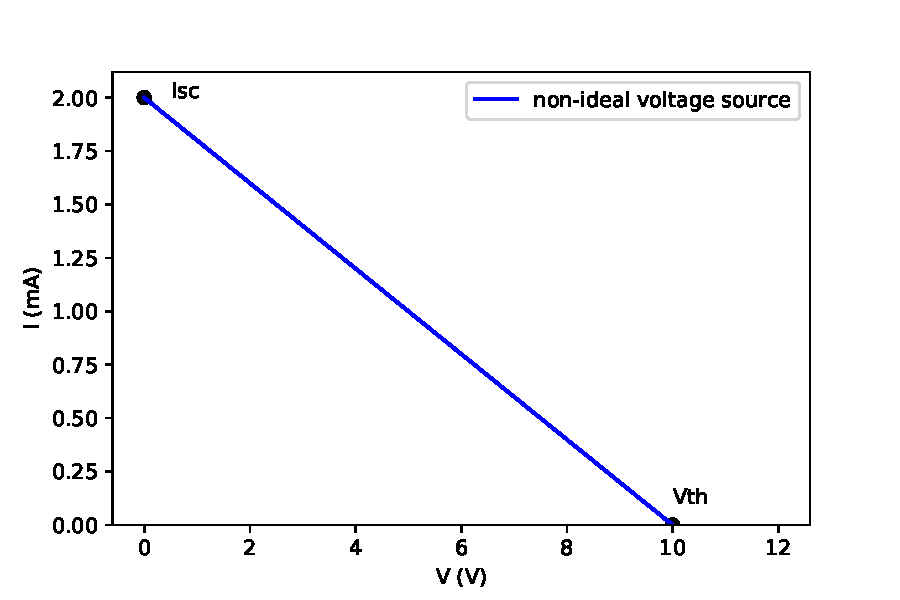
\includegraphics[height=0.3\textheight]{figs/thevenin.pdf} 
\caption{ The source IV curve for an arbitrary two terminal network.}
\label{fig:thevenin_source}
\end{center}
\end{figure}

\begin{figure}[htbp]
\begin{center}
\begin{tabular}{cc}
\begin{circuitikz}[line width=1pt]
\draw (0,0) node[right]{A} to[short,o-*] ++(-1.0,0) coordinate(X) to[resistor,l_=$R_8$] ++(0,2.0)
to[resistor,l_=$R_7$] ++(0,2.0) to[resistor,l_=$R_6$] ++(0,2.0) to[short,-o] ++(1.0,0) node[right]{B};
\draw (X) to[resistor,l=$R_5$] ++(-2.0,0) coordinate(X);
\draw (X) to[voltage source,bipoles/length=1.5cm,l=$V_1$] ++(0,+2.0) coordinate(X) to[resistor,l=$R_4$,*-*] ++(2.0,0);
\draw (X) to[voltage source,bipoles/length=1.5cm,l=$V_2$] ++(0,+2.0) coordinate(X) to[resistor,l=$R_3$,*-*] ++(2.0,0);
\draw (X) to[resistor,l=$R_1$] ++(0,+2.0) to[resistor,l=$R_2$,-*] ++(2.0,0);
\end{circuitikz} &
\begin{circuitikz}[line width=1pt]
\draw (0,0) node[right]{A} to[short,o-] ++(-1.0,0) to[voltage source,bipoles/length=1.5cm,l=$V_{\rm th}$] ++(0,+2.0) 
to[R, l=$R_{\rm th}$] ++(0,+2.0) to[short, i>=$I$,-o] ++(1.0,0) node[right]{B};
\end{circuitikz} \\
(a) & (b) \\
\end{tabular}
\caption{ Two-terminal network diagrams for (a) a fairly complicated network, and (b) it's Thevenin equivalent.}
\label{fig:thev_eg}
\end{center}
\end{figure}


\section{Exercises}

\begin{enumerate}

\item Derive Equations~\ref{eqn:rseries} and \ref{eqn:rparallel}.

\item Derive Equation~\ref{eqn:idivider}.

\item Show that the power consumed by a resistor of resistance $R$ conducting a current $I$ is:
\begin{displaymath}
P = I^2R
\end{displaymath}

\item Show that the power consumed by a resistor of resistance $R$ held at a voltage $V$ is:
\begin{displaymath}
P = V^2/R
\end{displaymath}

\item Using circuit analysis, determine the operating point (Q) of the
  circuit in Fig.~\ref{fig:vrr_iv} and compare with the value you read
  off from the plot.

%\item Draw the $IV$ curve for an ideal voltage source and a
%  short-circuit.  Do they intersect?  What do you suppose would happen
%  if you attempted to short-circuit an ideal voltage source?  Now draw
%  an open circuit ($I=0$).  What is the operating point of a voltage
%  source with it's terminals left open?  


\item We already discussed ideal voltage sources which will provide
  any necessary current to maintain a constant voltage across two
  terminals.  Another linear circuit element source is an ideal
  current source, which provides any necessary voltage to maintain a
  constant current through its two terminals.  Sketch the $IV$ curve
  for a constant voltage source and a constant current source.  Ideal
  voltage sources have zero intrinsic resistance.  What intrinsic
  resistance does an ideal current source have?  (Hint: look at the IV
  curve and recall the relationship between slope and resistance.)
  One way to make a current source is to place a very large resistor
  in series with a very large voltage source.  Is this consistent with
  your answer?

%\item Draw the $IV diagrams$ for an ideal current source and an open-circuit (I=0).  Do they intersect?  What do you suppose would happen if you attempted to leave the terminals of an ideal voltage source open?  Now draw a short circuit.  What is the operating point of a voltage source with it's terminals left open?  

\item Find the Thevenin Equivalent voltage, resistance, and short-circuit current for the following two terminal network:
\begin{center}
\begin{circuitikz}[line width=1pt]
\draw (0,0) node[right]{A} to[short,o-*] coordinate(X) ++(-1.0,0) coordinate(X) to[resistor,l_=$R_2$] ++(0,2.0) to[short,*-o] ++(1.0,0) node[right]{B};
\draw (X) to[short,*-] ++ (-2.0,0) to[voltage source,bipoles/length=1.5cm,l=$V_1$] ++(0,+2.0) to[resistor,l=$R_1$] ++(2.0,0);
\end{circuitikz} \\
\end{center}
Leave your answer in terms of $R_1$, $R_2$, and $V_1$.

\item Find the Thevenin Equivalent voltage and resistance for the following two-terminal network:
\begin{center}
\begin{circuitikz}[line width=1pt]
\draw (0,0) node[right]{A} to[short,o-] ++(-1.0,0) coordinate(X) 
to[voltage source,bipoles/length=1.5cm,l=$V_3$] ++(0,2.0) to[R,l=$R_3$] ++(0,2.0) 
to[short,-o] ++(1.0,0) node[right]{B};
\draw (X) to[short,*-] ++(-2.0,0) coordinate(X) 
to[voltage source,bipoles/length=1.5cm,l=$V_2$] ++(0,2.0) to[R,l=$R_2$] ++(0,2.0) 
to[short,-*] ++(2.0,0);
\draw (X) to[short,*-] ++(-2.0,0) coordinate(X) 
to[voltage source,bipoles/length=1.5cm,l=$V_1$] ++(0,2.0) to[R,l=$R_1$] ++(0,2.0) 
to[short,-*] ++(2.0,0);
\end{circuitikz} \\
\end{center}
Leave your answer in terms of $R_1$, $R_2$, $R_3$, $V_1$, $V_2$ and $V_3$.  

\item  When you ask why they are late with their share of the rent (again), your roommate explains that they would like to invest the money into buying inexpensive force sensors for about \$10 each.  They think they can use these to make cheap electronic drum kits and sell them at a profit.   The idea is to connect a force sensor acting as a switch between a $9~\rm V$ battery and an old $50~\rm \Omega$ (load resistance) speaker.  Each customer will supply their own battery and speaker, and the wire will be pilfered from Physics 80 lab.  While perusing the specs for the force sensor, you notice that they have a typical source resistance of about $100~\rm k\Omega$.    Model the proposal as a DC voltage divider, which is sufficient analysis to see what a terrible design your roommate has concocted.  What's the maximum voltage you would see across the speaker given the source resistance and load resistance?  What's the maximum power that would be consumed by the speaker?  Compare this with the power consumed by the speaker at typical operating voltages of at least $1~\rm V$.   Whatever you do, do not leave the room without the rent money in cash!!!

\end{enumerate}

